\documentclass[11pt]{beamer}
\usetheme{CambridgeUS}
\usepackage[utf8]{inputenc}
\usepackage[UKenglish]{babel}
\usepackage[T1]{fontenc}
\usepackage{amsmath}
\usepackage{amsfonts}
\usepackage{amssymb}
\usepackage{graphicx}
\author[A.D.]{Anthony Debruyn\\~\\\small{\textit{Sup. Gaëtan Podevijn}}}
\title{Wysiwyd}
%\setbeamercovered{transparent} 
\setbeamertemplate{navigation symbols}{} 
\logo{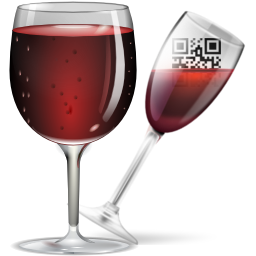
\includegraphics[scale=0.1]{Images/iconh.png}} 
\institute[ULB]{Université Libre de Bruxelles} 
%\date{} 
%\subject{}


\AtBeginSection[]
{
  \begin{frame}
  \frametitle{Contents}
  \tableofcontents[currentsection, hideothersubsections, pausesubsections]
  \end{frame} 
}


\setbeamercolor{section number projected}{bg=red,fg=white}
\setbeamertemplate{itemize item}{$\color{orange}\blacktriangleright$}
\setbeamertemplate{itemize subitem}{$\color{orange}\blacktriangleright$}

\begin{document}

\begin{frame}
\titlepage
\end{frame}

\begin{frame}
\tableofcontents
\end{frame}

%-----------------------------------------------------------------------
%	Introduction
%-----------------------------------------------------------------------
\section{Introduction}
\begin{frame}{Problem}

\begin{itemize}
	\item Manage a large collection of bottles
	\item Ergonomic, easy, aesthetic
	\item Take into account large number of wine properties
	\item Easy bottle finding, addition
	\item Save a picture of the bottle
\end{itemize}

\end{frame}

\begin{frame}{Existing Solutions}
\begin{description}
	\item[Vivino] Internet connection to work, to recognise a bottle. Cellar management is not the main purpose of the app.
	\item[Eurocave] No quick bottle recognition, lots of bugs.
	\item[Wine Cellar] Bottle properties not fully represented.
\end{description}
\end{frame}

%-----------------------------------------------------------------------
%	Solution
%-----------------------------------------------------------------------
\section{Solution}

\begin{frame}{Propositions}
\begin{itemize}
	\item Wine cellar app, focus on what is important.
	\item Quick bottle recognition without internet connection.\\
	Use of new, user friendly technologies to do so: NFC \& QR/bar code.
	\item A lot of properties to edit.
	\item Intuitive, simple, user friendly.
\end{itemize}

\center $\Rightarrow$ Wysiwyd
\center \emph{What you scan is what you drink.}
\end{frame}

\logo{}

\begin{frame}
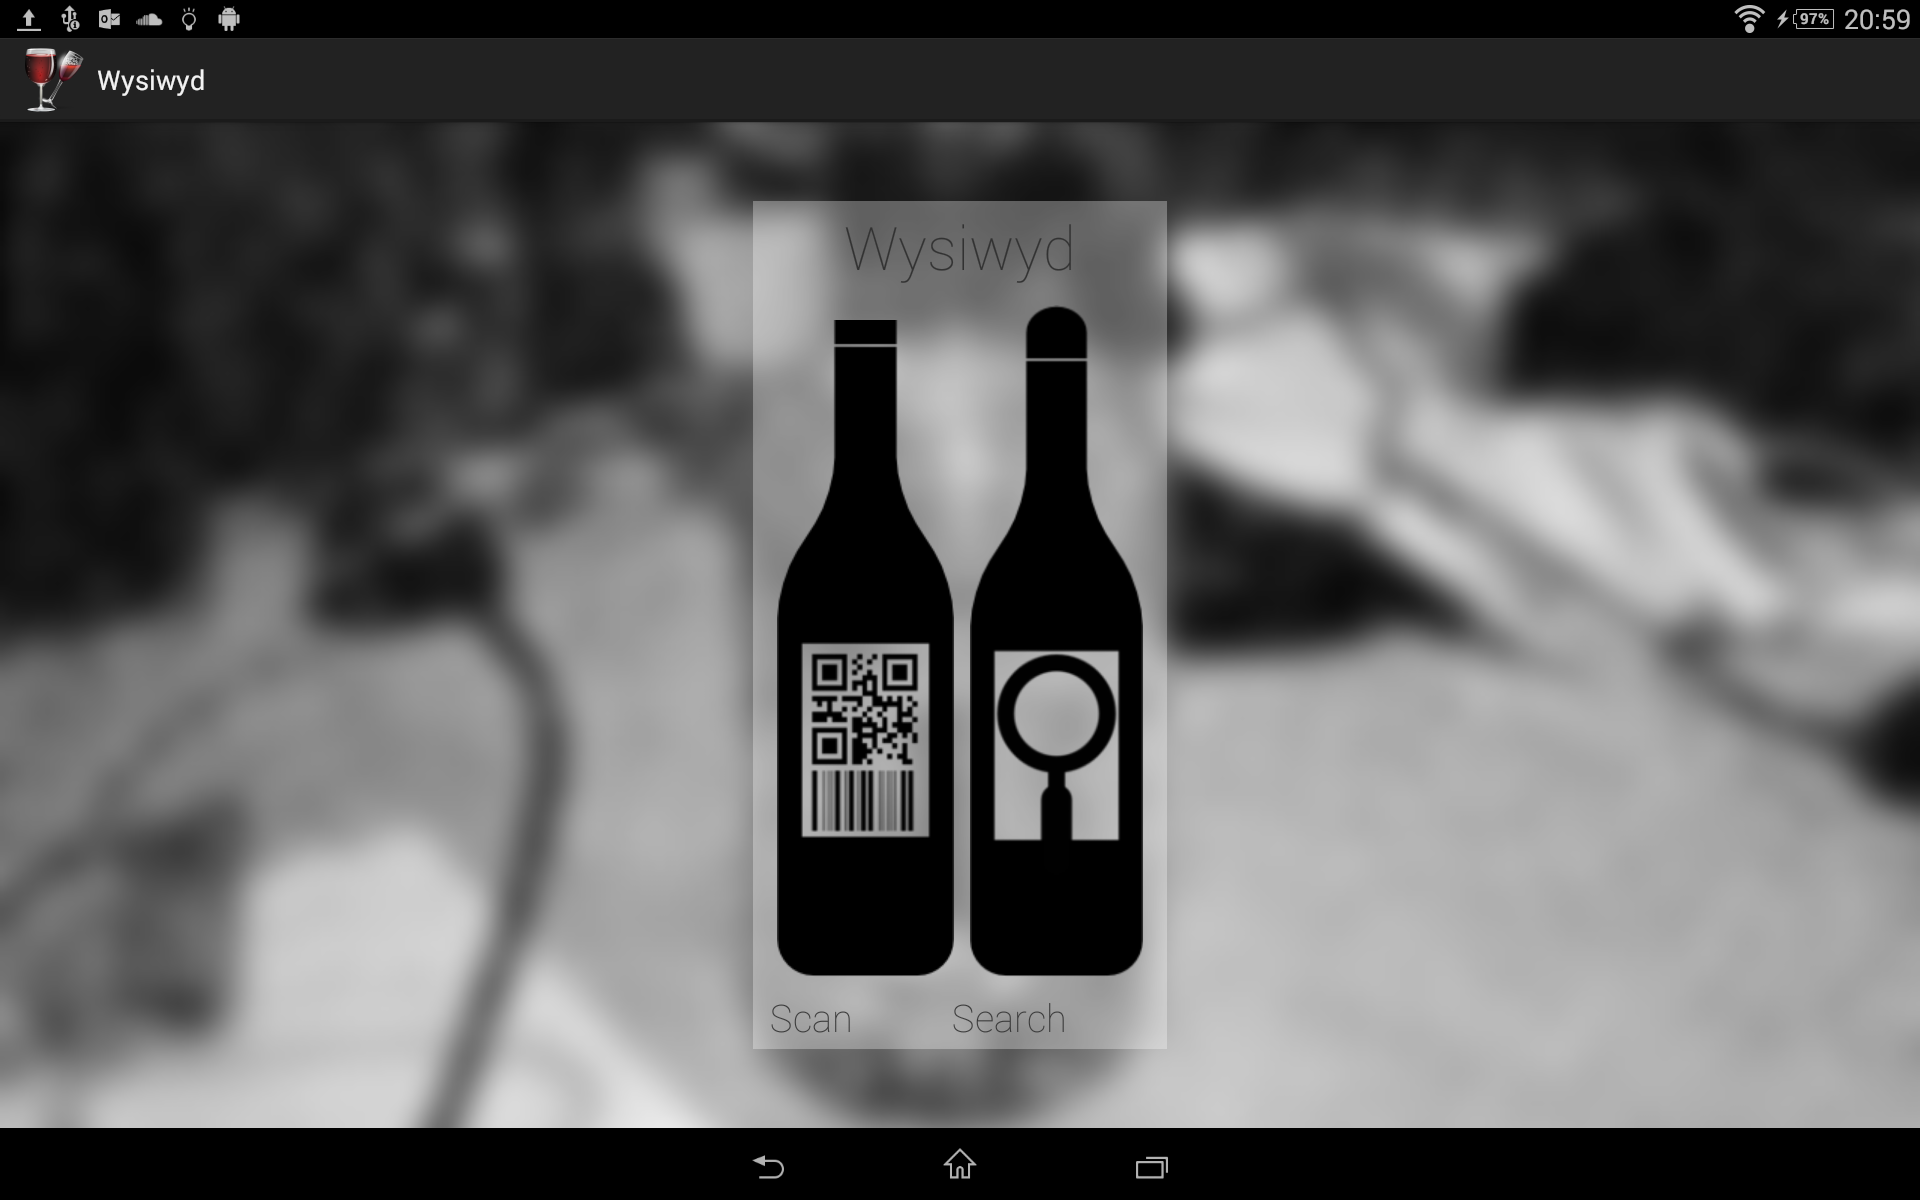
\includegraphics[scale=0.18]{Images/MainActivity.png}
\end{frame}

\begin{frame}
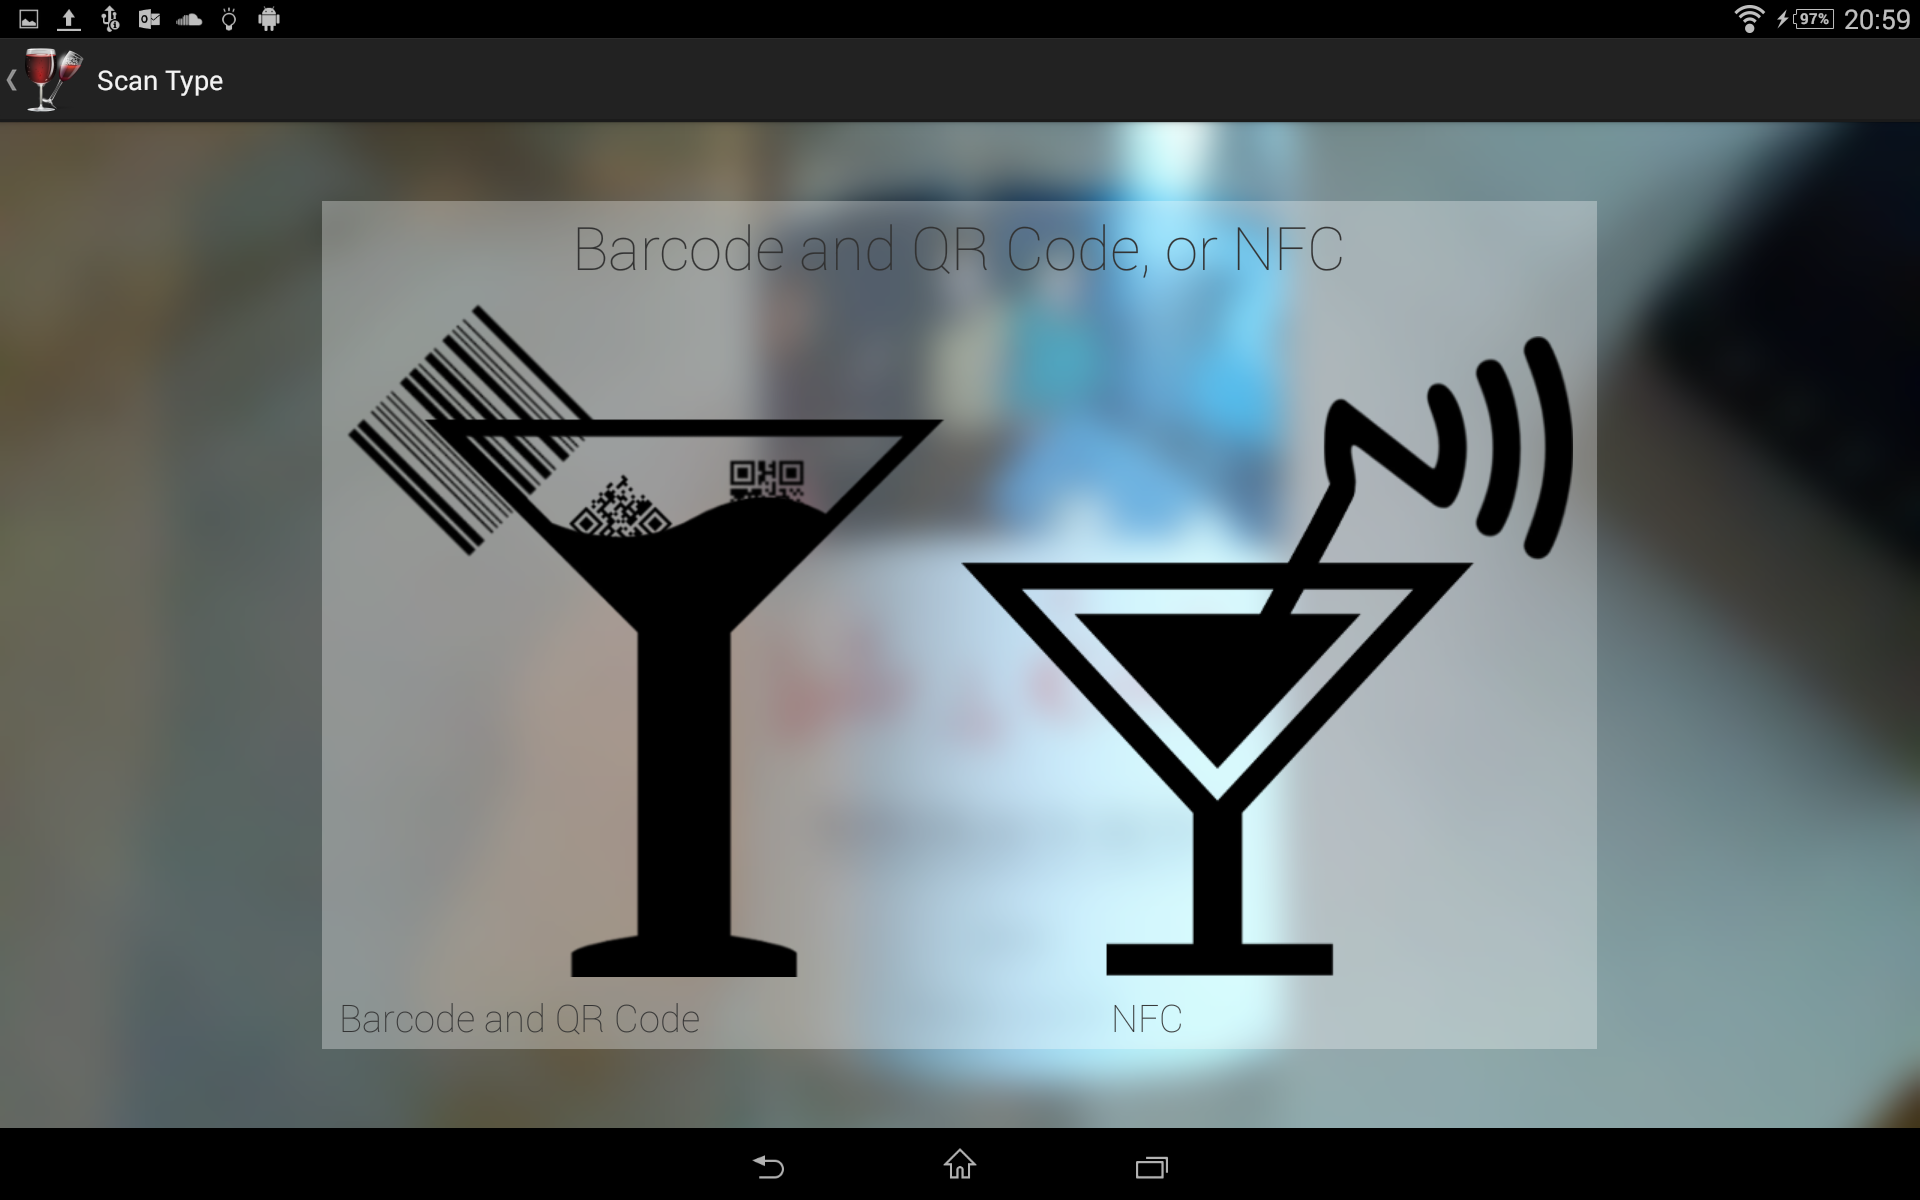
\includegraphics[scale=0.18]{Images/ScanChoice.png}
\end{frame}

\begin{frame}
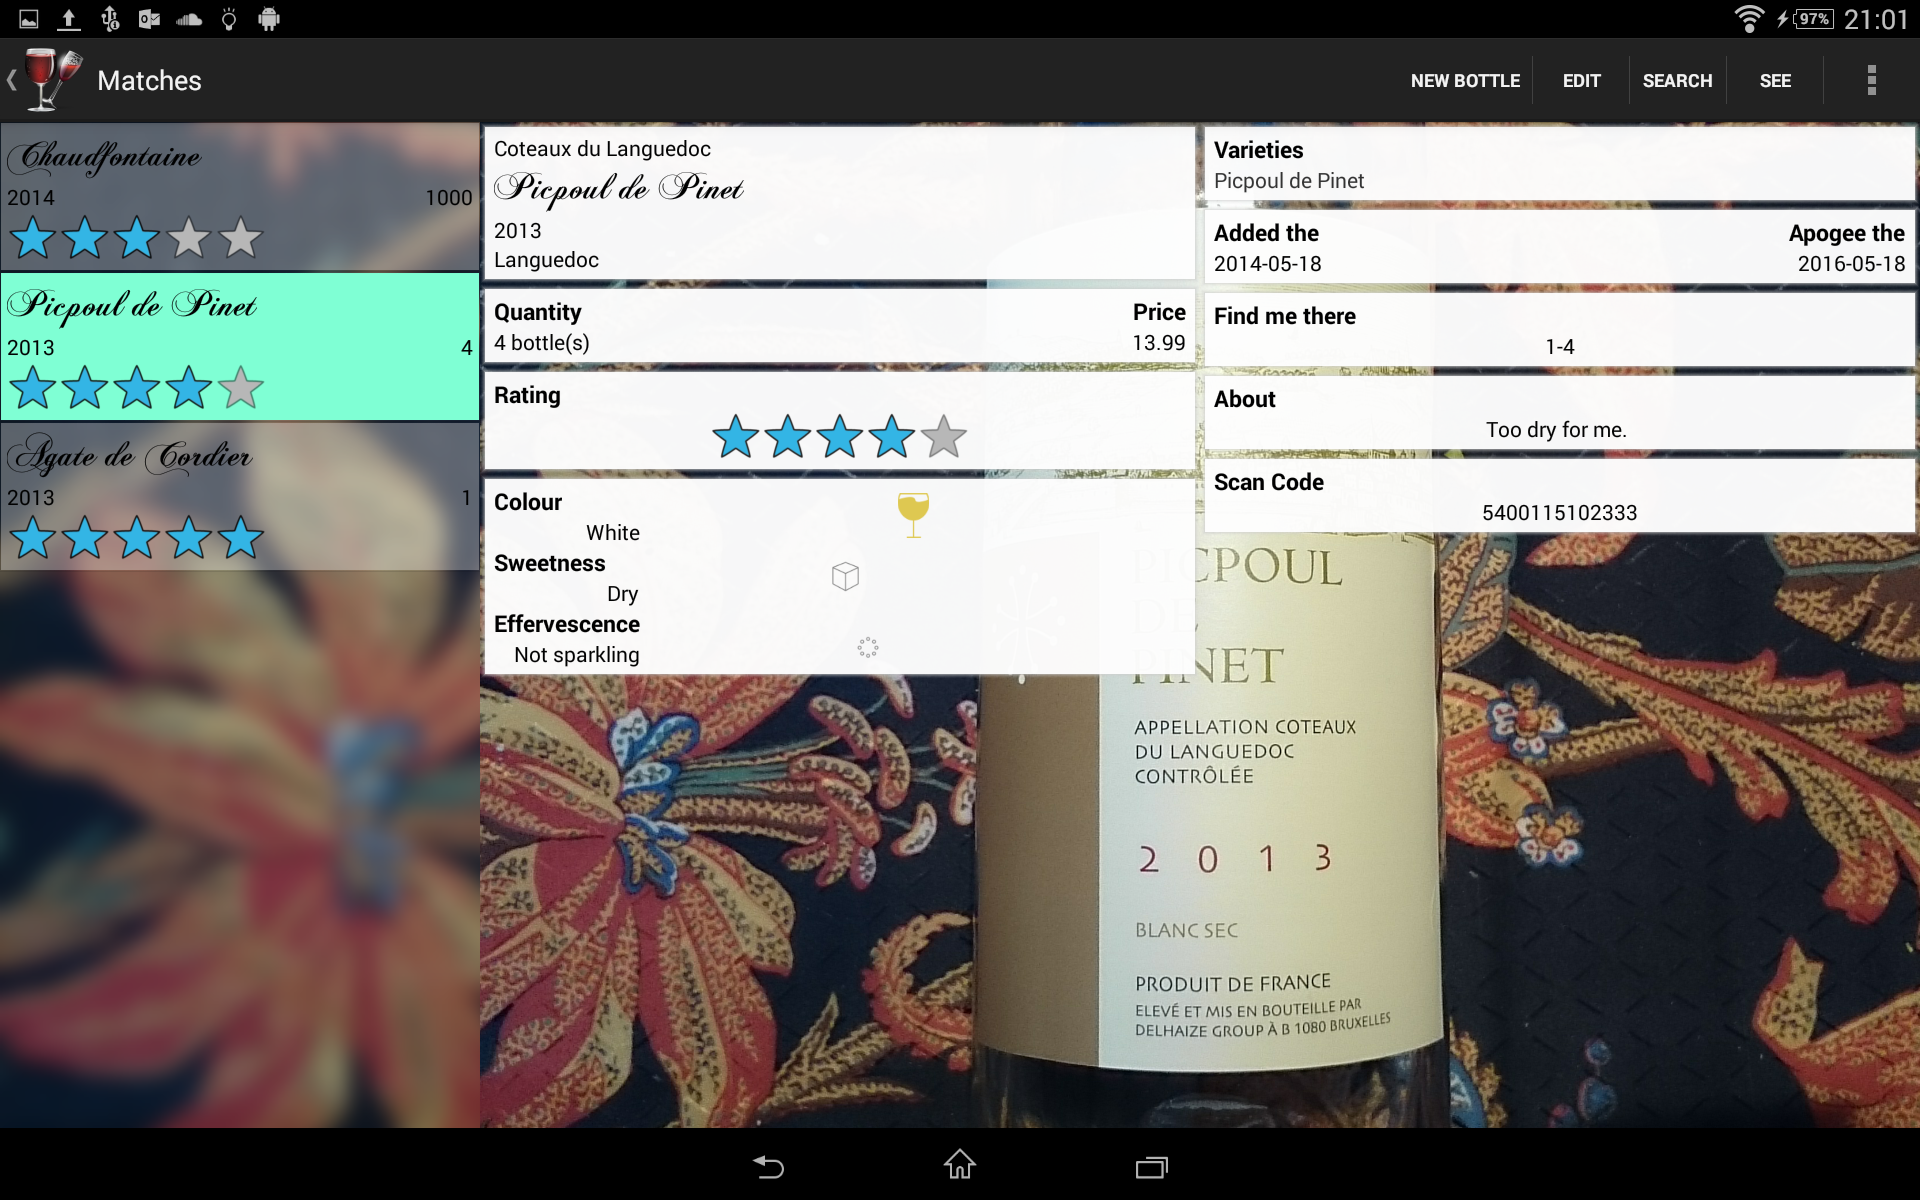
\includegraphics[scale=0.18]{Images/ResultsActivity.png}
\end{frame}

\logo{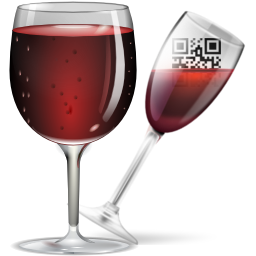
\includegraphics[scale=0.1]{Images/iconh.png}}


%-----------------------------------------------------------------------
%	Demo
%-----------------------------------------------------------------------
\section{Demo}

\begin{frame}{Demo}
	\center \Huge{Demo}
\end{frame}
%-----------------------------------------------------------------------
%	Future Work & Limitations
%-----------------------------------------------------------------------
\section{Future Work \& Limitations}

\begin{frame}{Future Work \& Limitations}
\begin{itemize}
	\item Cloud database
	\item Use support library to access below 4.0 API market share
	\item Notification system
	\item Exportation of the database
	\item Advanced "find me there" functionality
	\item Port to other systems
	\item Pages in search results
\end{itemize}
\end{frame}

%-----------------------------------------------------------------------
%	Conclusion
%-----------------------------------------------------------------------
\section{Conclusion}

\begin{frame}{Conclusion}
\begin{itemize}
	\item Easy, aesthetic way to manage large wine cellar
	\item Wine properties $\Rightarrow$ complete personalisation of bottles
	\item Adding, Finding bottles made simple with NFC \& QR/bar codes
\end{itemize}
\end{frame}

\end{document}